\chapter{Introduction}
\label{ch:intro}

The ability to engineer and manipulate quantum states lies at the heart of modern atomic physics experiments using ultracold gases \cite{Davis1995,Anderson1995,Bradley1995,DeMarco1999,Lang2008,Ni2008}. Two important tools for this pursuit are Feshbach resonances \cite{Chin2010,Kohler2006} and optical lattices \cite{Bloch2008}. This proposal will detail our recent work building and characterizing a three-dimension optical lattice for use with ultracold and quantum degenerate gases of neutral strontium. Furthermore, we will present the first experiment we hope to pursue with the optical lattice; the creation of Feshbach molecules using an optical Feshbach resonance. We will also briefly discuss other future plans such as the production of highly excited ground state Sr$_2$ dimers through adiabatic internal state transfer.

Should probably mention somewhere that this is long-range PA, in contrast to short-range stuff being explored now.

Julienne form of the corss section 6.16 in CM. Discuss how important the phase space density is, the timescale for interactions, and the complex 

\cite{Aman2018}

\section{Few-body physics}
\label{sec:few-body}

field of photoassociation in ultracold gases, wherein studies of molecular structure have revealed the most accurate descriptions of atomic interactions and have become a fundamental probe of the ultracold toolbox \cite{Jones2006}.

\section{Halo molecules}
\label{sec:halo}

Mostly studied in helium

Comes from bound state of the dirac potential. Unsure how much detail I want right here

Check out CM Juleinne pg 229. He has a ref

\section{Properties of strontium}
\label{sec:sr}

	\begin{figure}
		\centerline{
		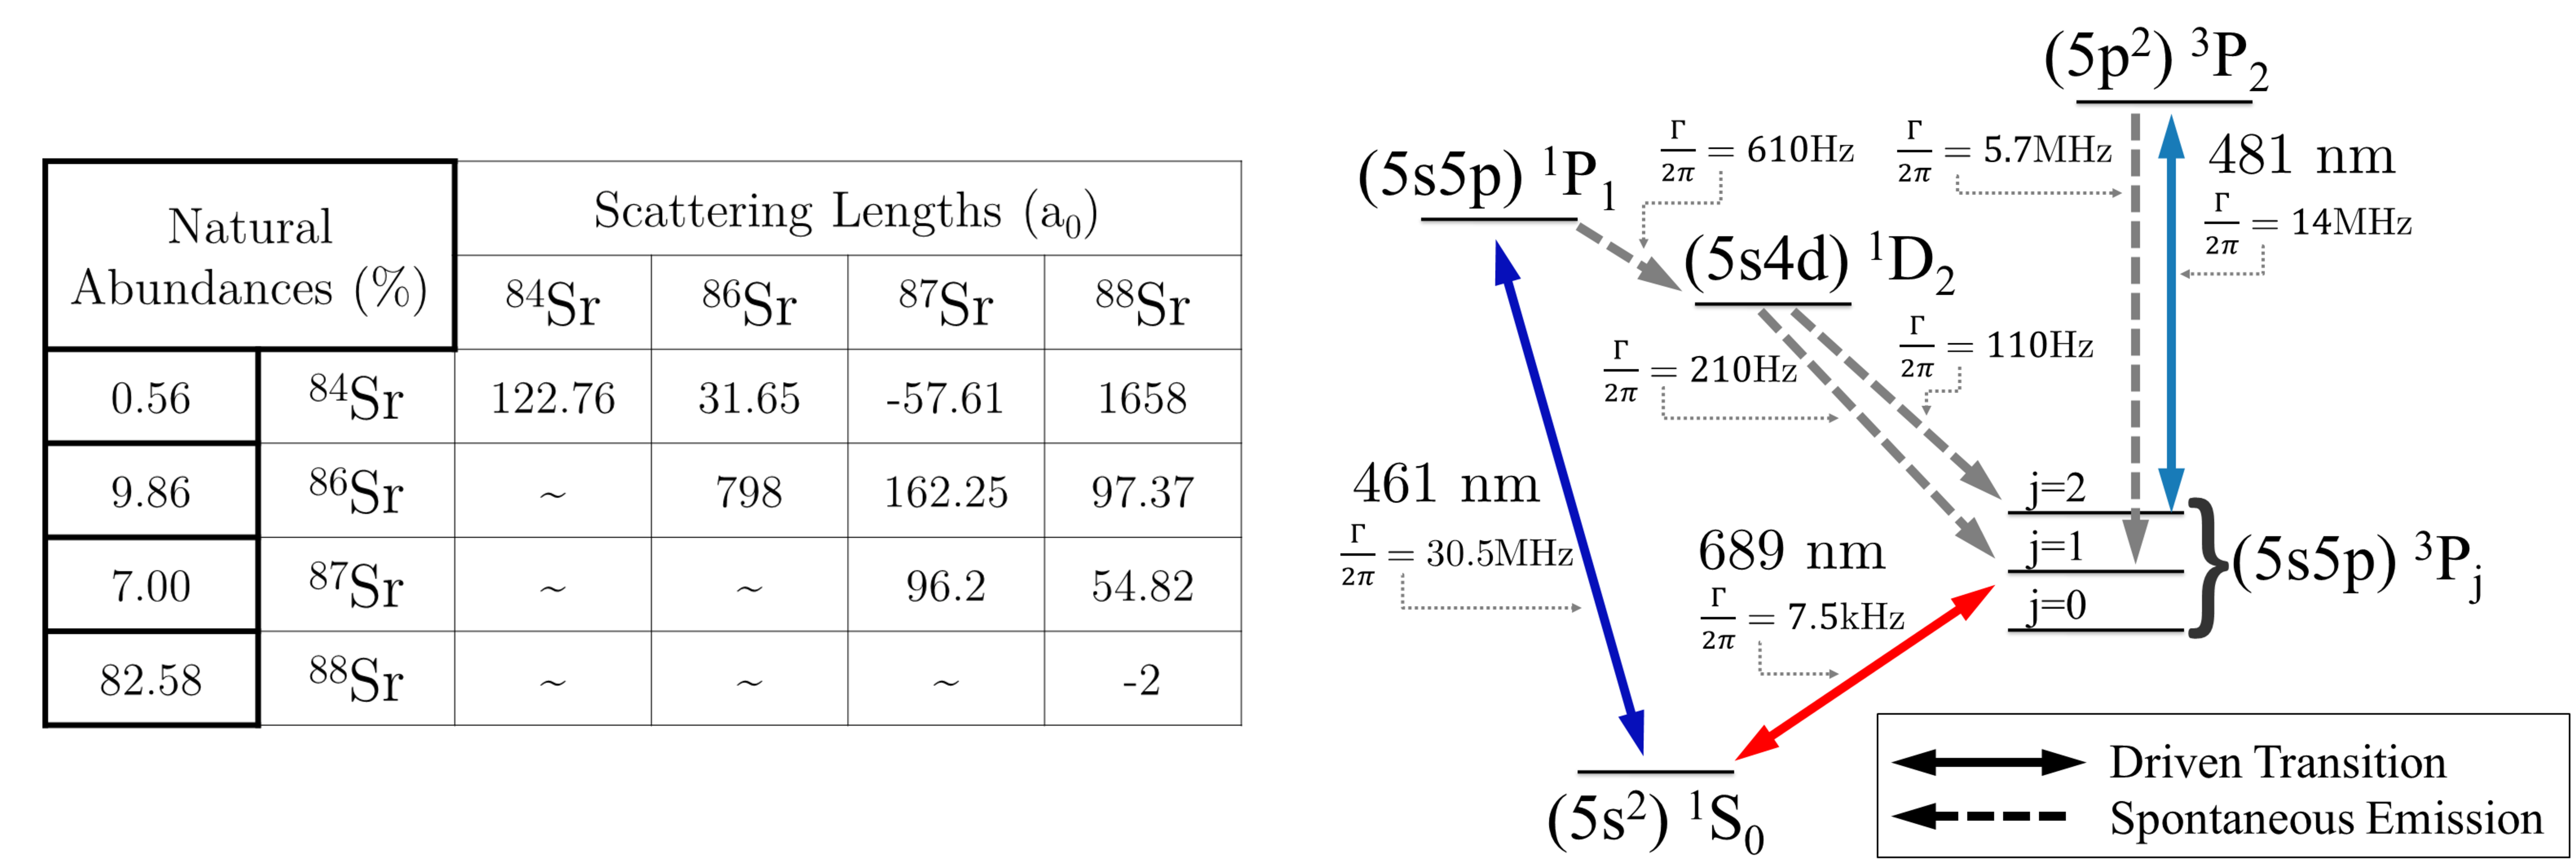
\includegraphics[height=0.25\textheight]{Fig1_strontium_properties.pdf}}
		\caption{Properties of strontium. Left: Natural abundances and s-wave scattering lengths for all mixtures of Sr. Right: Simplified energy level diagram of Sr showing the relevant states used for trapping and cooling of the atomic gas}
	\end{figure} 
The experiments in this proposal will be realized using an ultracold gas of atomic strontium. Fig.\;\ref{fig:energy_level_diagram} shows all of the stable isotopes of strontium, their natural abundance, as well as their inter-particle scattering lengths. The isotopic differences in strontium have important implications for their use in certain experiments. For example, none of the bosonic isotopes of strontium ($^{88}$Sr, $^{86}$Sr, or $^{84}$Sr) display hyperfine structure since they have no nuclear spin, $\vec{I}=0$. However, the fermionic isotope $^{87}$Sr has a large nuclear spin, $\vec{I}=9/2$, which makes it an ideal candidate for exploring exotic phases of quantum magnetism \cite{Beverland2016,Cazalilla2014,Chen2015}. In the studies presented in this proposal, we are sensitive to the isotopic shifts of the bosonic photoassociation lines along the $^1S_0\!\rightarrow\!^3P_1$ transition as well as the various interspecies scattering lengths.

\begin{figure}
\label{fig:energy_level_diagram}
	\centerline{
	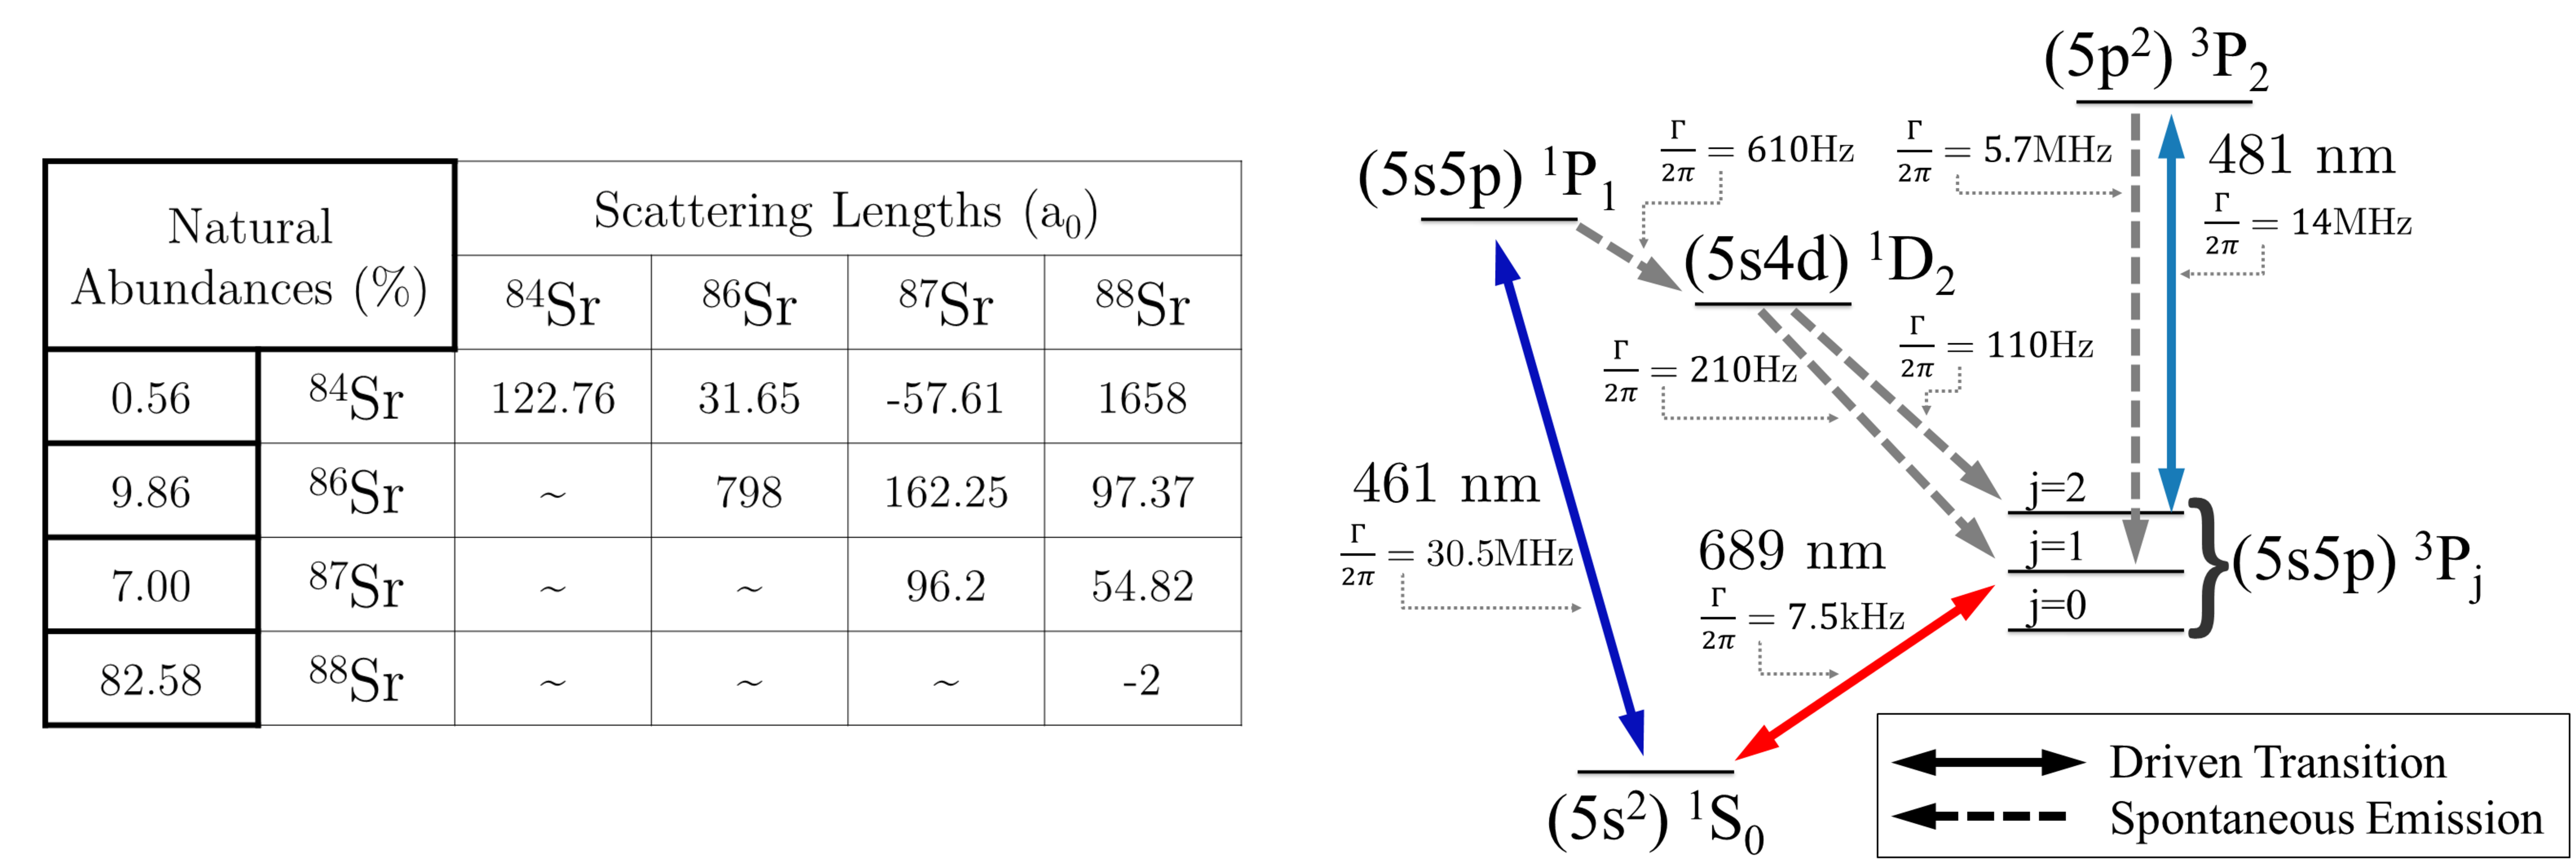
\includegraphics[height=0.25\textheight]{strontium_properties.pdf}}
	\caption{Properties of strontium}{Properties of strontium. Left: Natural abundances and s-wave scattering lengths for all mixtures of Sr. Right: Simplified energy level diagram of Sr showing the relevant states used for trapping and cooling of the atomic gas}
\end{figure} 

\section{Thesis Outline}
\label{sec:outline}

"Lorem ipsum dolor sit amet, consectetur adipiscing elit, sed do eiusmod tempor incididunt ut labore et dolore magna aliqua. Ut enim ad minim veniam, quis nostrud exercitation ullamco laboris nisi ut aliquip ex ea commodo consequat. Duis aute irure dolor in reprehenderit in voluptate velit esse cillum dolore eu fugiat nulla pariatur. Excepteur sint occaecat cupidatat non proident, sunt in culpa qui officia deserunt mollit anim id est laborum."


\begin{equation} 
\label{eq:1dlattice}
		 V(x) = V_{lat} \; \sin^2(k_L x)
\end{equation}



